\documentclass[UTF8,titlepage]{ctexart}
\usepackage{amsmath,amssymb,amsthm,amsfonts,amscd}
\usepackage{fontspec}
\setmainfont{Times New Roman}
\usepackage{graphicx}
\usepackage{titlesec}
\usepackage{makecell}
\usepackage{longtable}
\usepackage{xcolor}
\usepackage{tcolorbox}
\usepackage{soul}
\usepackage{adjustbox}
\usepackage{tcolorbox}
\usepackage{enumerate}
\usepackage{pdfpages}
\usepackage{float}
\usepackage{colortbl}
\usepackage{tabularx}
\usepackage{multirow}
\usepackage{pgfplots}
\usepackage{minted}
\numberwithin{figure}{section}
\usepackage[left=1.25in,right=1.25in,%
top=1in,bottom=1in]{geometry}
\usepackage{color}
\titleformat{\section}
  {\raggedright\LARGE\bfseries}{\thesection}{1em}{}
\begin{document}
\title{{\Huge{\textbf{程序设计实践课程报告}}}}
\author{姓名:赵伯远 \\ 学号:211440128 \\班级:人工智能2101 \\ 序号:75}
\date{\today}
\maketitle
\tableofcontents
\clearpage

\section{课题一:运动会分数统计}

\subsection{任务描述}

参加运动会有 n 个学校,学校编号为 1……n。比赛分成m 个男子项目和w个女子项目。项目编号为男子:1$\sim$m,女子:m+1$\sim$m+w。不同的项目取前五名或前三名积分;取前五名的积分分别为:7、5、3、2、1,前三名的积分分别为:5、3、2;哪些项目取前五名或前三名由学生自己设定。(m<=20, n<=20)
 
\subsection{功能要求}

\begin{enumerate}
    \item 可以输入各个项目的前三名或前五名的成绩;
    \item 能统计各学校总分;
    \item 可以按学校编号、学校总分、男女团体总分排序输出;
    \item 可以按学校编号查询学校某个项目的情况;
    \item 可以按项目编号查询取得前三或前五名的学校。
    \item 允许用户指定某项目采取其他名次的取法。
    \end{enumerate}

\subsection{需求分析}
此程序主要实现的功能有:
\begin{enumerate}
    \item 收集每个学校的男女团队在各项目中的得分。
    \item 按照学校编号、总分、男女团体得分进行排序。
    \item 提供查询功能:查询指定学校在指定项目中的得分,查询指定项目取得前几名的学校。
\end{enumerate}

首先需要构建顺序表储存相关信息,如参赛学校的名称,获得的分数,比赛
项目,及其相关的赋分规则,以及参赛选手信息。然后需要输入比赛相关信息,
如参数学校,比赛项目的相关信息,至此基础信息完备。在项目结束后输入相关
获奖人员信息即可按照积分给出各种排名。

程序流程图如下:
\begin{figure}[H]
\centering
 \resizebox{0.5\textwidth}{!}{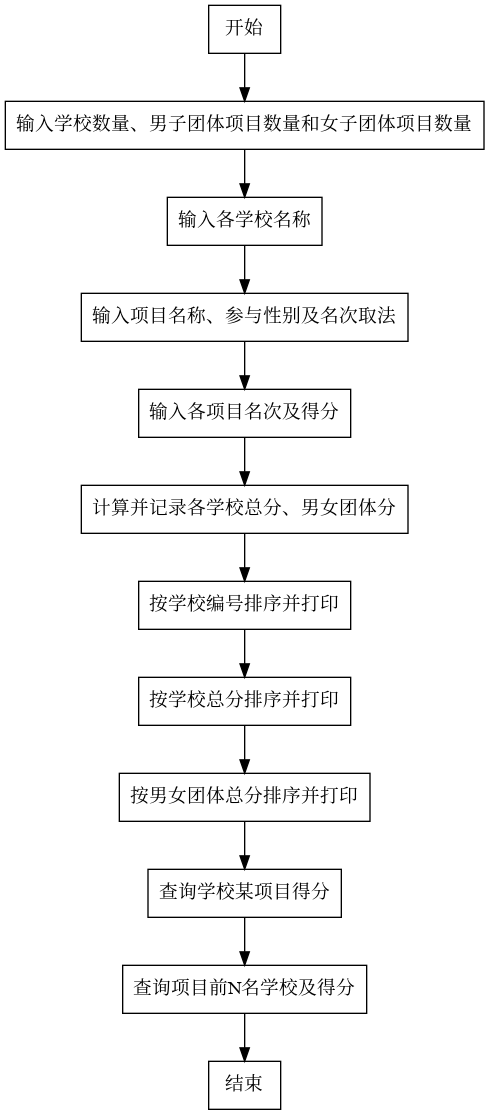
\includegraphics{./fig/program_flowchart.png}}
 \caption{程序流程图}
 \label{}
\end{figure}

\subsection{概要分析}
\begin{figure}[H]
\centering
 \resizebox{1\textwidth}{!}{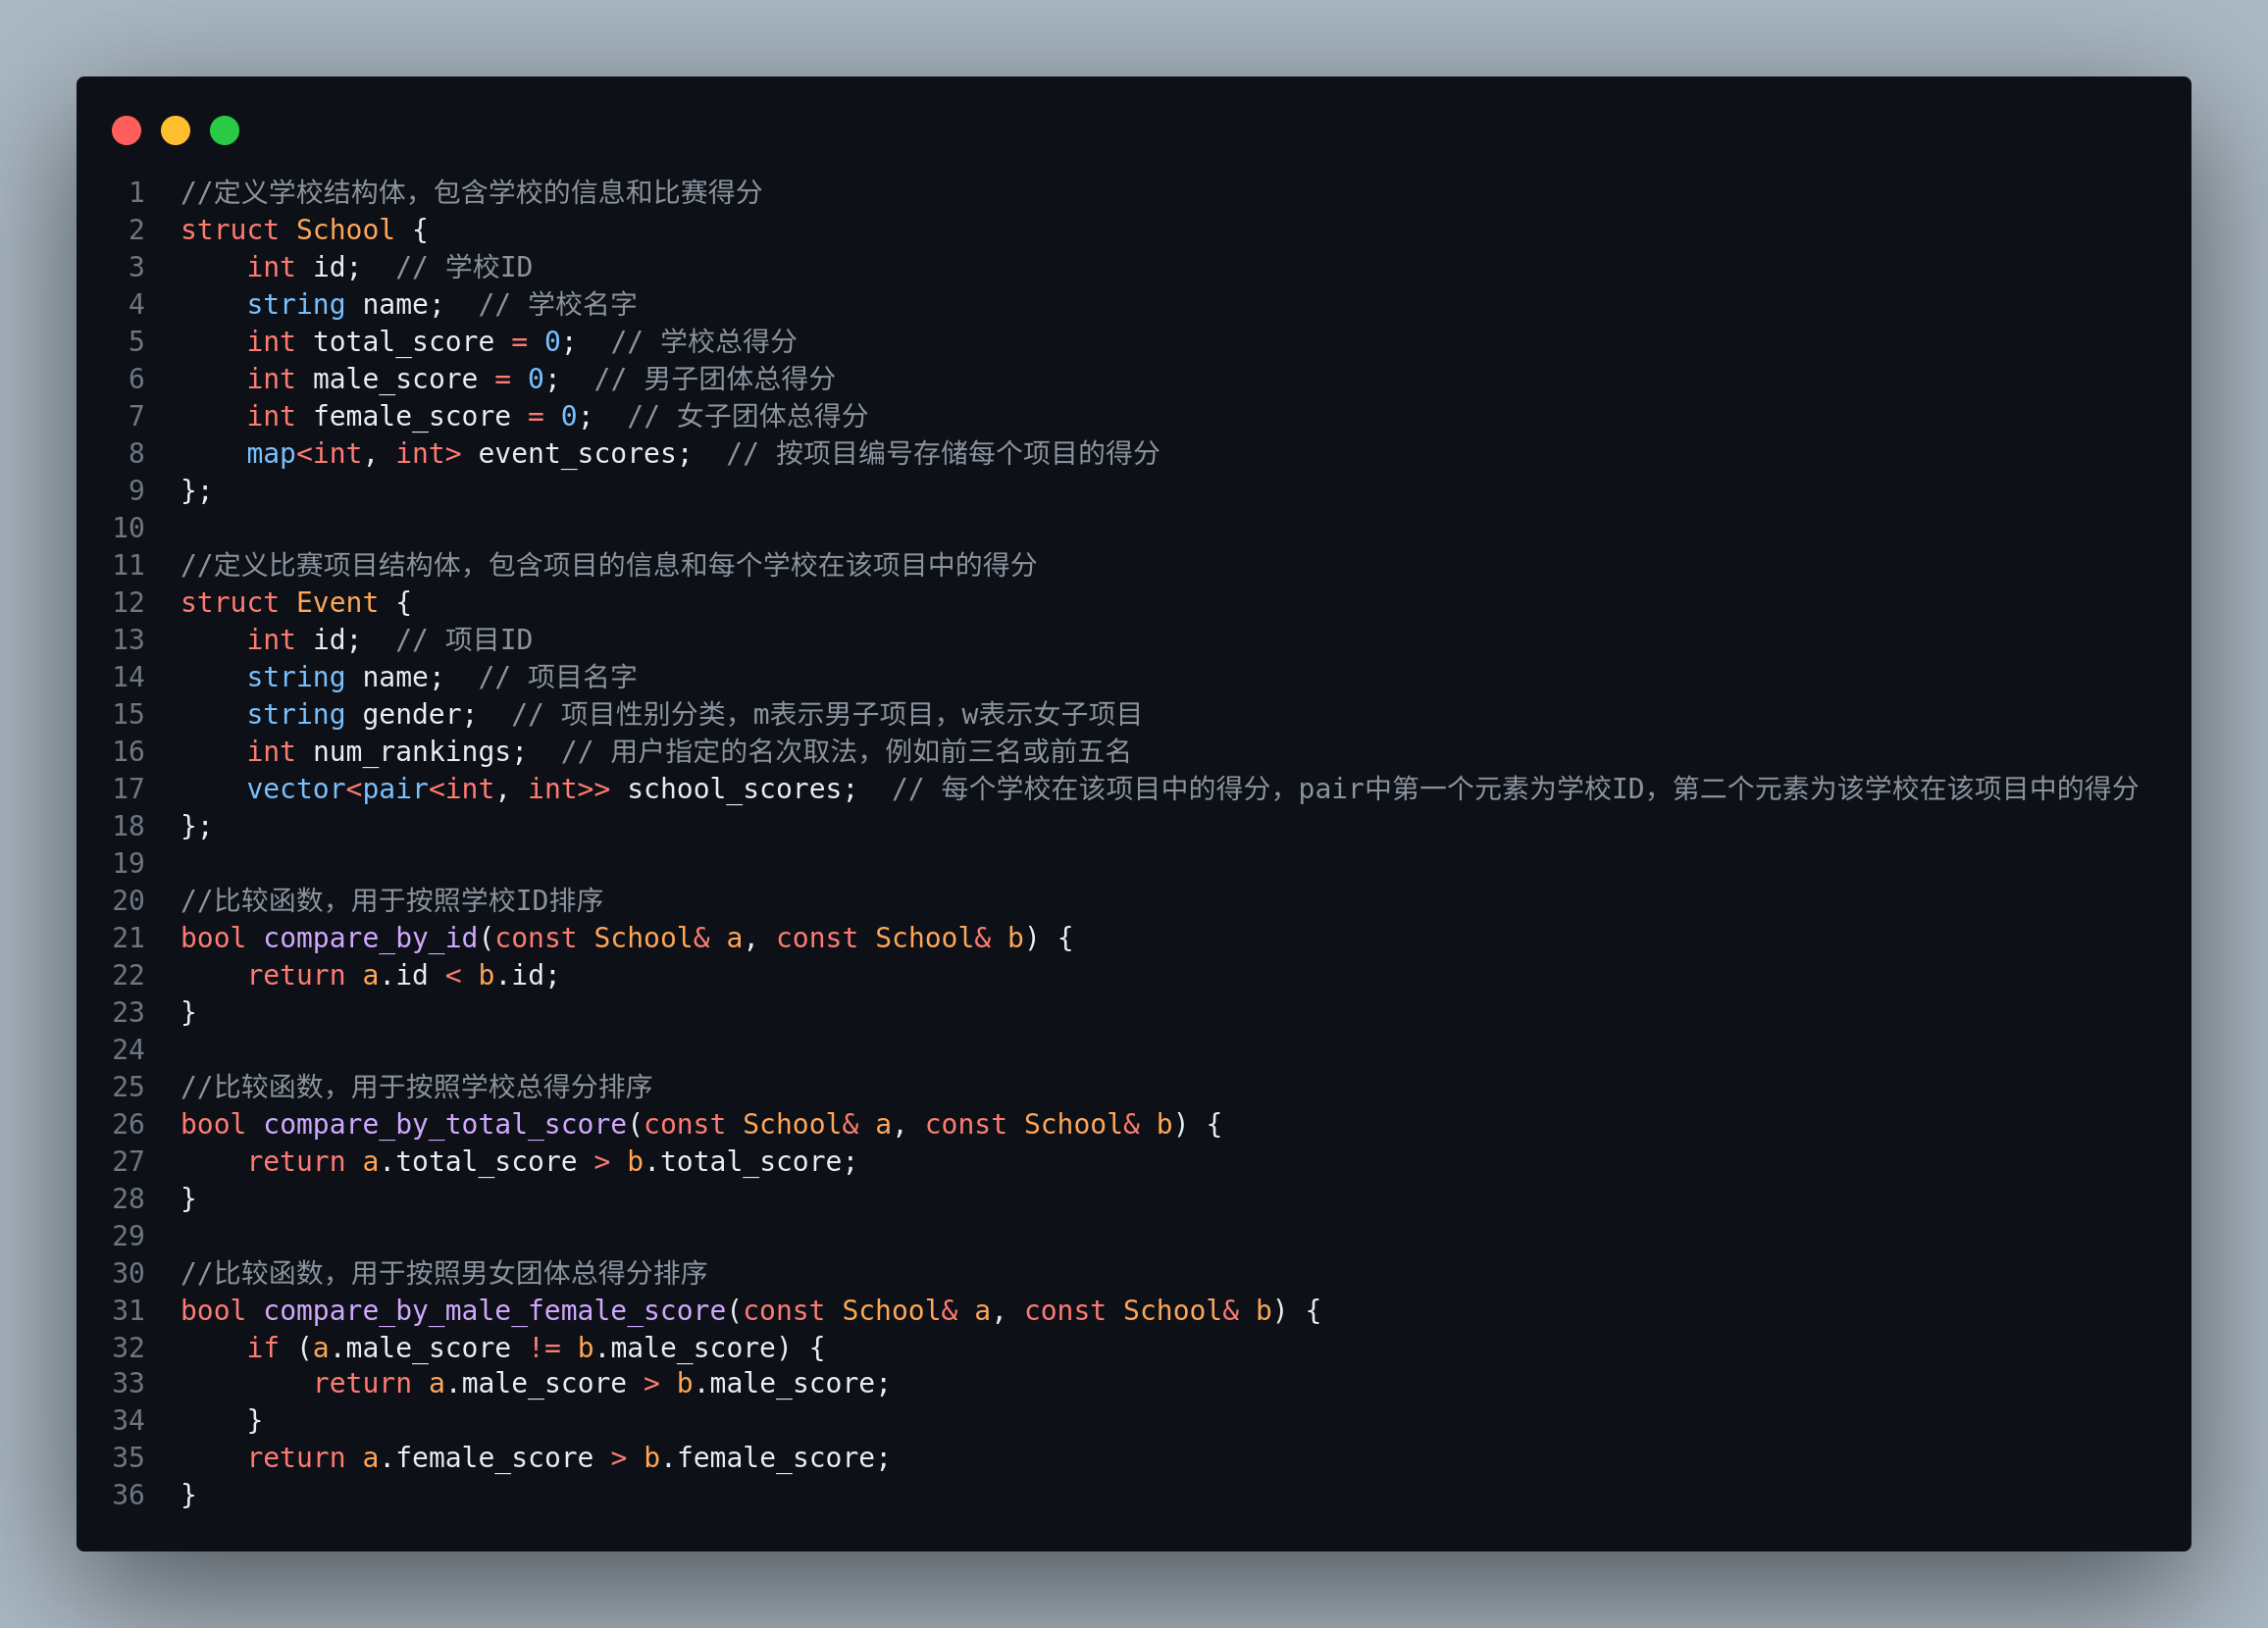
\includegraphics{./fig/struct.png}}
 \caption{程序基本结构体\&基本函数}
 \label{}
\end{figure}

\subsection{详细分析}
完整代码如下:
\begin{minted}[linenos]{c++}
#include <iostream>
#include <vector>
#include <map>
#include <algorithm>
#include <string>

using namespace std;

//定义学校结构体,包含学校的信息和比赛得分
struct School {
    int id;  // 学校ID
    string name;  // 学校名字
    int total_score = 0;  // 学校总得分
    int male_score = 0;  // 男子团体总得分
    int female_score = 0;  // 女子团体总得分
    map<int, int> event_scores;  // 按项目编号存储每个项目的得分
};

//定义比赛项目结构体,包含项目的信息和每个学校在该项目中的得分
struct Event {
    int id;  // 项目ID
    string name;  // 项目名字
    string gender;  // 项目性别分类,m表示男子项目,w表示女子项目
    int num_rankings;  // 用户指定的名次取法,例如前三名或前五名
    vector<pair<int, int>> school_scores;  // 每个学校在该项目中的得分,
                                           //pair中第一个元素为学校ID,
                                           //第二个元素为该学校在该项目中的得分
};

//比较函数,用于按照学校ID排序
bool compare_by_id(const School& a, const School& b) {
    return a.id < b.id;
}

//比较函数,用于按照学校总得分排序
bool compare_by_total_score(const School& a, const School& b) {
    return a.total_score > b.total_score;
}

//比较函数,用于按照男女团体总得分排序
bool compare_by_male_female_score(const School& a, const School& b) {
    if (a.male_score != b.male_score) {
        return a.male_score > b.male_score;
    }
    return a.female_score > b.female_score;
}


int main() {
    int n, m, w;
    cout << "请输入学校数量、男子团体项目数量、女子团体项目数量:" << endl;
    cin >> n >> m >> w;
    cout << "请输入学校名称:" << endl;
    vector<School> schools(n);
    for (int i = 0; i < n; ++i) {
        schools[i].id = i + 1;
        cin >> schools[i].name;
    }
    cout << "请输入项目名称, 参与性别及名次取法:" << endl; // 让用户指定每个项目的名次取法
    vector<Event> events(m + w);
    for (int i = 0; i < m + w; ++i) {
        events[i].id = i + 1;
        // 获取用户指定的名次取法
        cin >> events[i].name >> events[i].gender 
            >> events[i].num_rankings; 
    }

    for (auto& event : events) {
        for (int i = 0; i < event.num_rankings; ++i) { // 根据用户指定的名次取法计算学校得分
            int school_id, score;
            cout<< "请输入项目 " << event.name << " 的第 " 
                << i + 1 << " 名学校编号和得分:" << endl;
            cin >> school_id >> score;
            event.school_scores.push_back({school_id, score});

            School& school = schools[school_id - 1];
            school.total_score += score;
            if (event.gender=="m") {
                school.male_score += score;
            } else {
                school.female_score += score;
                cout<< school.female_score<<endl;
            }
            school.event_scores[event.id] = score;
        }
    }
    // 输出学校编号排序
    sort(schools.begin(), schools.end(), compare_by_id);
    cout << "按学校编号排序:" << endl;
    for (const auto& school : schools) {
        cout << school.name << " (编号: " << school.id << ")" << endl;
    }
    cout << endl;

    // 输出学校总分排序
    sort(schools.begin(), schools.end(), compare_by_total_score);
    cout << "按学校总分排序:" << endl;
    for (const auto& school : schools) {
        cout << school.name << " (总分: " << school.total_score << ")" << endl;
    }
    cout << endl;

    // 输出男女团体总分排序
    sort(schools.begin(), schools.end(), compare_by_male_female_score);
    cout << "按男女团体总分排序:" << endl;
    for (const auto& school : schools) {
        cout << school.name << " (男子团队分数: " << school.male_score 
             << ", 女子团队分数: " << school.female_score << ")" << endl;
    }
    cout << endl;

    // 查询学校某个项目的情况
    int query_school_id, query_event_id;
    cout << "请输入查询的学校编号和项目编号:" << endl;
    cin >> query_school_id >> query_event_id;
    const School& query_school = schools[query_school_id - 1];
    auto it = query_school.event_scores.find(query_event_id);
    if (it != query_school.event_scores.end()) {
        cout << query_school.name << " 在项目 " << events[query_event_id - 1].name 
             << " 中的得分为: " << it->second << endl;
    } else {
        cout << query_school.name << " 在项目 " << events[query_event_id - 1].name 
             << " 中没有得分" << endl;
    }
    cout << endl;

    // 按项目编号查询取得前三或前五名的学校
    cout << "请输入要查询的项目编号:" << endl;
    int query_event_id2;
    cin >> query_event_id2;
    const Event& query_event = events[query_event_id2 - 1];

    cout << "在项目 " << query_event.name << " 中取得前" 
         << query_event.num_rankings << "名的学校有:" << endl;
    for (const auto& school_score : query_event.school_scores) {
        cout << schools[school_score.first - 1].name << " (得分: " 
             << school_score.second << ")" << endl;
    }

    return 0;
}


\end{minted}

\subsection{调试分析}
\begin{enumerate}
    \item 问题:在计算学校得分时,学校编号的索引与实际编号存在偏差。
    
          解决方案:在读取学校编号后,需要将其减1,以符合实际索引。
    

          \item 问题:按学校编号排序输出时,学校编号不是按照升序排列。
    
          解决方案:可以在排序函数sort(schools.begin(), schools.end(), compare\_by\_id)之前添加调用compare\_by\_id函数的输出语句,检查是否正确比较学校编号。
    \item 问题:程序无法正确查询取得前三或前五名的学校。
    
          解决方案:根据用户输入的项目编号,获取该项目的参与学校列表,并根据学校的得分进行排序。然后输出前三或前五名学校的名称和得分。确保在处理边界情况时进行适当的错误检查。

\end{enumerate}

\subsection{用户手册}
\begin{enumerate}
    \item 演示程序的运行环境为 Ubuntu 20.04 系统,GCC 9.4.0\ x86\_64-linux-gnu.。执行指令为
    
    cd "/media/zby/SSD数据盘/Program-Practice/Sport/" \&\& g++ main.cpp -o main \&\& "/media/zby/SSD数据盘/Program-Practice/Sport/"main

    \begin{figure}[H]
    \centering
     \resizebox{0.75\textwidth}{!}{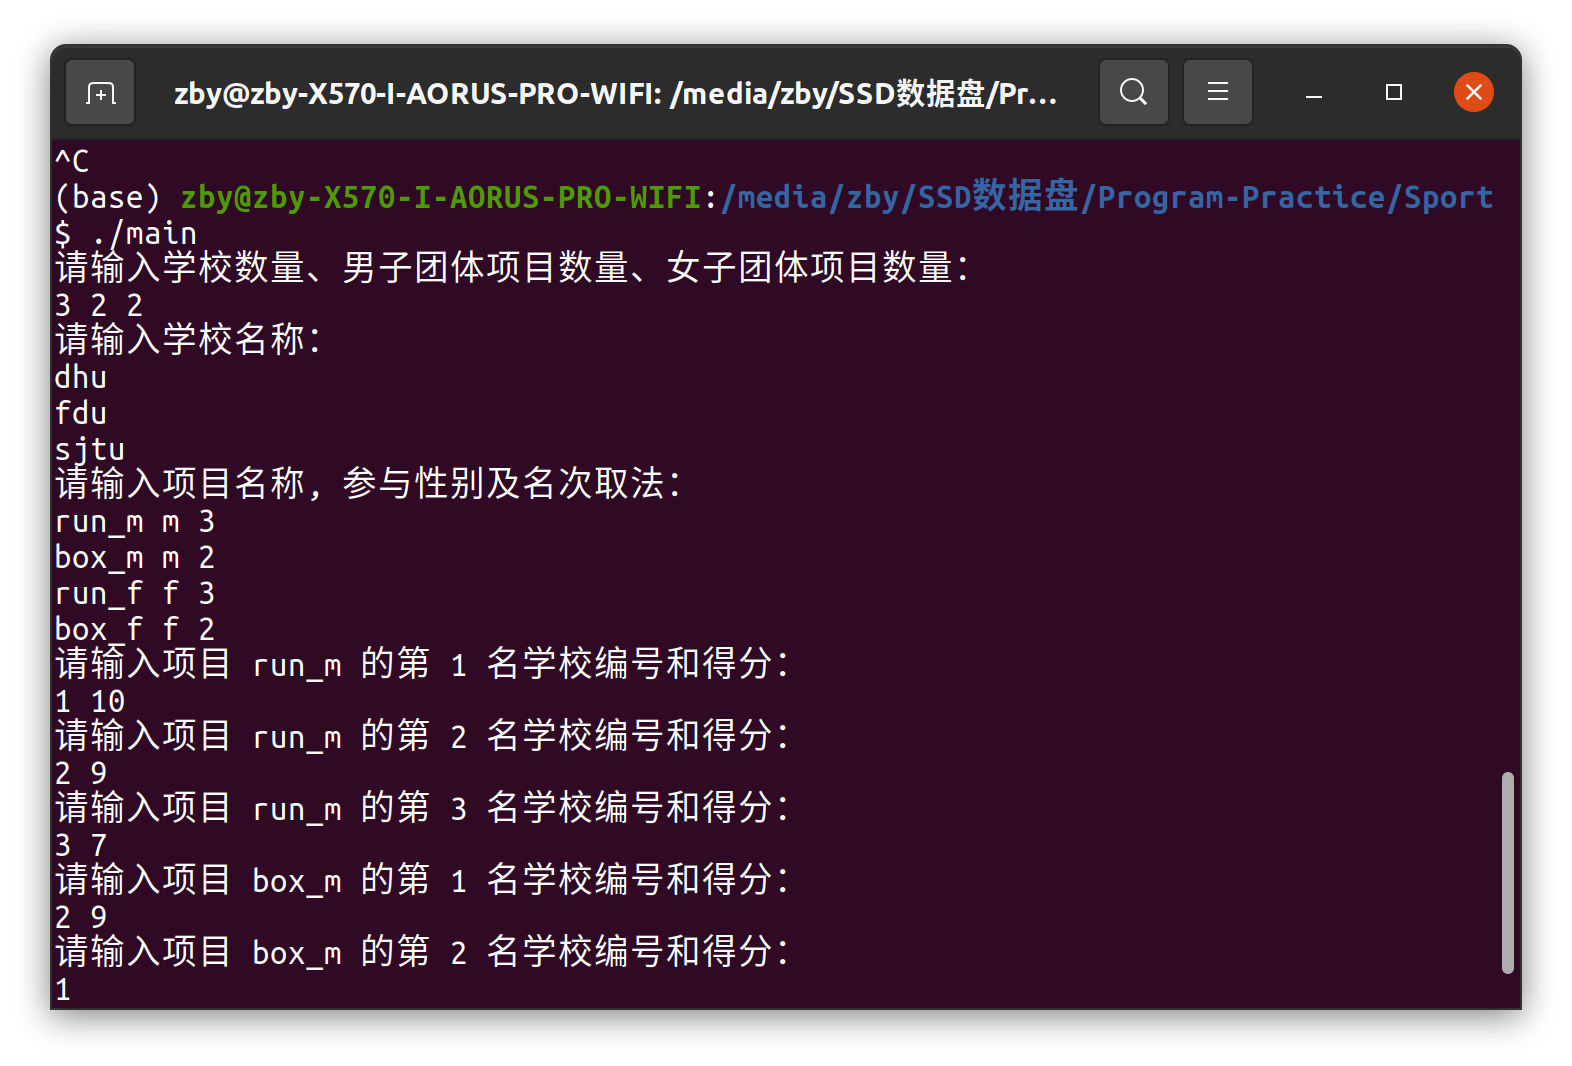
\includegraphics{./fig/sport1.png}}
     \caption{初始界面}
     \label{}
    \end{figure}

    \begin{figure}[H]
    \centering
     \resizebox{0.75\textwidth}{!}{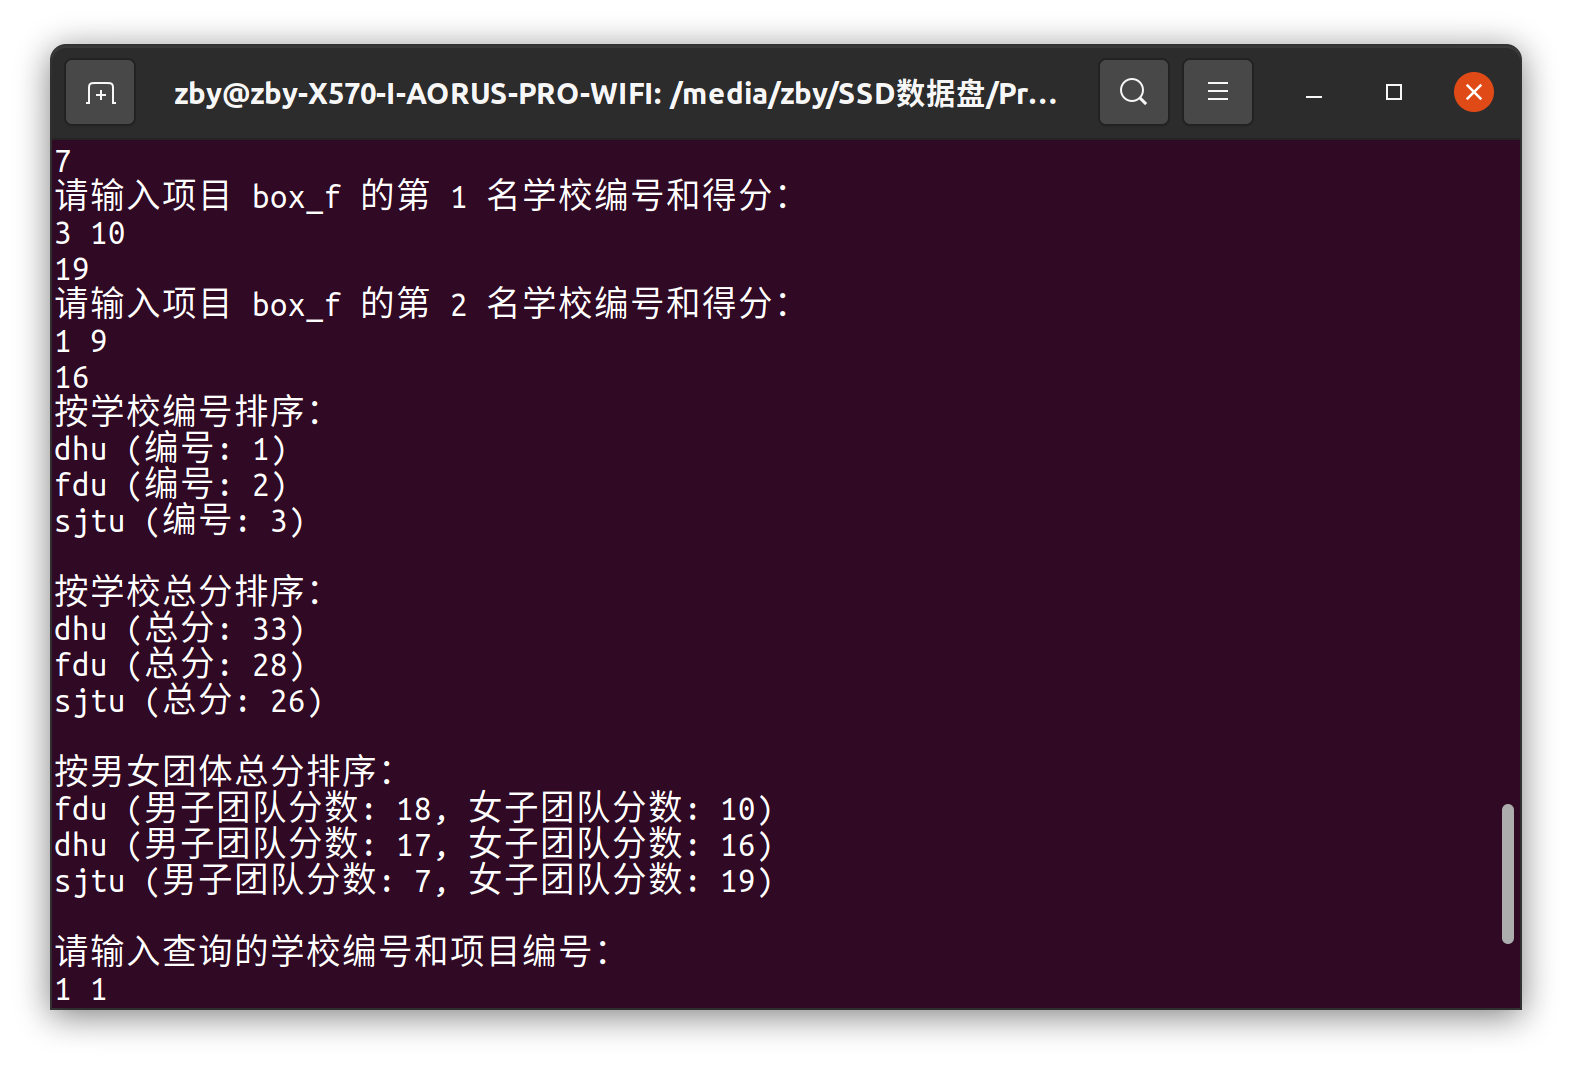
\includegraphics{./fig/sport2.png}}
     \caption{输入数据}
     \label{}
    \end{figure}

    \begin{figure}[H]
    \centering
     \resizebox{0.75\textwidth}{!}{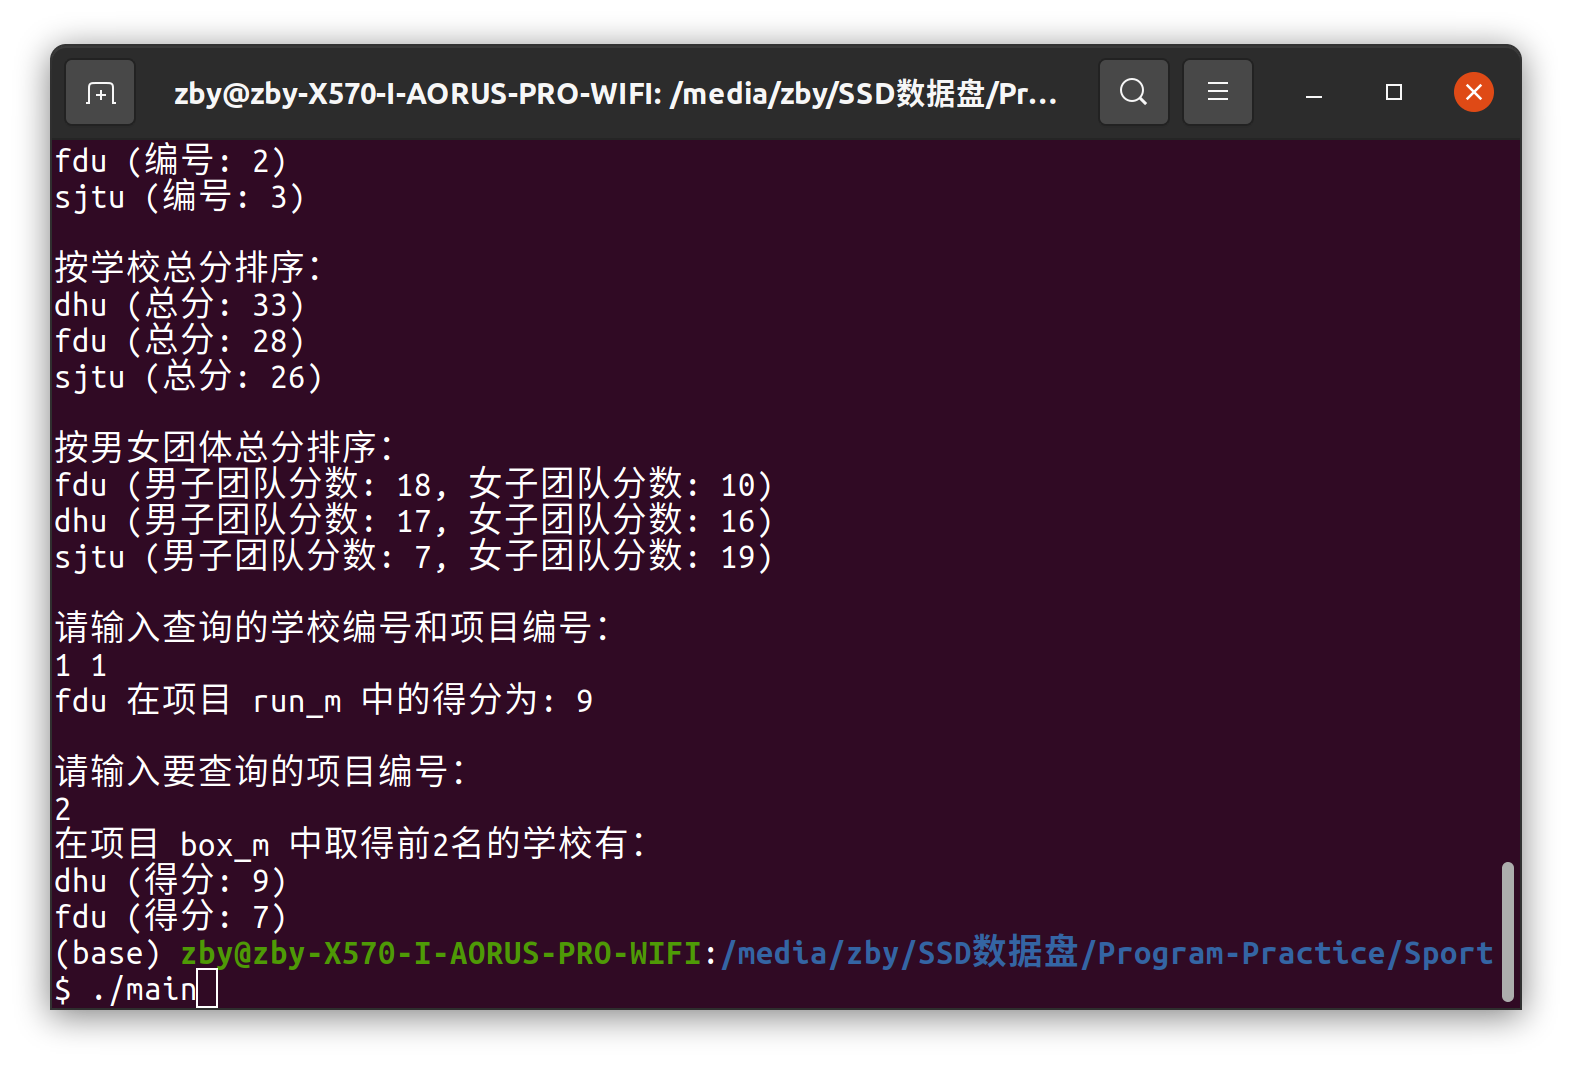
\includegraphics{./fig/sport3.png}}
     \caption{查询操作}
     \label{}
    \end{figure}
\end{enumerate}
\subsection{总结}
本次实验我不拘泥于顺序结构的实现,同时去了解了STL中的map和set容器的使用,以及对于迭代器的使用。在实验过程中,我对于STL中的map和set容器的使用有了更深的理解。同时,我也对于STL中的sort函数有了更深的理解。
\clearpage
\section{课题二:停车场管理系统}
\subsection{任务描述}
设计一个停车场管理系统,模拟停车场的运作,此程序具备以下功能:
\begin{enumerate}
    \item[(1)] 若车辆到达,则显示汽车在停车场内或者便道上的停车位置;
    \item[(2)] 若车辆离去,则显示汽车在停车场内停留的时间和应缴纳的费用(在便道上停留的时间不收费)
\end{enumerate}

\subsection{基本要求}
\begin{enumerate}
    \item 要求以栈模拟停车场,以队列模拟车场外的便道,按照从终端读入和输
    入数据序列进行模拟管理。
    \item 要求处理的数据元素包括三个数据项:汽车“到达”或“离去”信息,
    汽车牌照号码及到达或离去的时刻。
    \item 要求栈以顺序结构实现,队列以链表实现。
\end{enumerate}

\subsection{需求分析}
主要流程为由用户输入进入停车场的车辆的信息,例如车牌号和进入时间以及离开时间,然后程序会自动生成所需要缴纳的费用。

\begin{figure}[H]
\centering
 \resizebox{0.75\textwidth}{!}{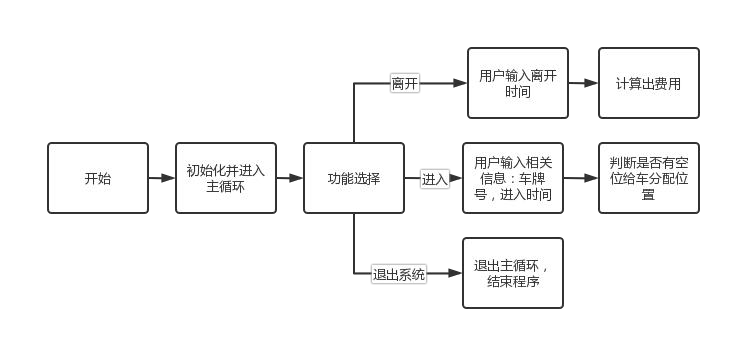
\includegraphics{./fig/parking_1.png}}
 \caption{程序流程图}
 \label{}
\end{figure}
由于没有外部的辅助设备,帮忙输入相关信息,这里让用户输入的方式来进
行完成。

\subsection{概要设计}
\begin{minted}[linenos]{c++}

    typedef struct {
        int hour;
        int min;
      } time;
      typedef struct {
        int num;
        int position;
        time t;
        float money;
      } Car;
      typedef struct Node {
        Car data;
        struct Node *next;
      } CQueueNode;
      typedef struct {
        Car elem[NUM + 1];
        int top;
      } Stack;
      typedef struct {
        CQueueNode *front;
        CQueueNode *rear;
      } LinkQueue;
      void InitQueue(LinkQueue *Q);
      // 初始化队列
      int EnterQueue(LinkQueue *Q, Car *t); // 进队
      void InitStack(Stack *S);
      // 初始化栈
      void Push(Stack *S, Car *r);
      // 压栈
      int IsEmpty(Stack *S);
      // 判断栈空
      int IsFull(Stack *S);
      // 判断栈满
      int GetTop(Stack *S, Car *n);
      int DeleteQueue(LinkQueue *Q, Car *x);
      void CarIn(Stack *S, LinkQueue *Q, Car *r);
      void CostCalculate(Car *r, int h, int m);
      void CarOut(Stack *S, Stack *S0, Car *r, LinkQueue *Q);
\end{minted}

\subsection{详细设计}
\begin{minted}[linenos]{c}
#include <stdio.h>
#include <stdlib.h>
#define NUM 20
typedef struct {
  int hour;
  int min;
} time;
typedef struct {
  int num;
  int position;
  time t;
  float money;
} Car;
typedef struct Node {
  Car data;
  struct Node *next;
} CQueueNode;
typedef struct {
  Car elem[NUM + 1];
  int top;
} Stack;
typedef struct {
  CQueueNode *front;
  CQueueNode *rear;
} LinkQueue;
void InitQueue(LinkQueue *Q);         // 初始化队列
int EnterQueue(LinkQueue *Q, Car *t); // 进队
void InitStack(Stack *S);             // 初始化栈
void Push(Stack *S, Car *r);          // 压栈
int IsEmpty(Stack *S);                // 判断栈空
int IsFull(Stack *S);                 // 判断栈满
int GetTop(Stack *S, Car *n);
int DeleteQueue(LinkQueue *Q, Car *x);
void CarIn(Stack *S, LinkQueue *Q, Car *r);
void CostCalculation(Car *r, int h, int m);
void CarOut(Stack *S, Stack *S0, Car *r, LinkQueue *Q);
int main(void) {
  int n, m, i = 1, j, flag = 0;
  Car c[10];
  Stack S, S0;
  LinkQueue Q;    // 便道
  InitStack(&S);  // 堆栈 S
  InitStack(&S0); // 临时堆栈 S0
  InitQueue(&Q);
  while (1) {
    printf("\t\t\t\t 欢迎停车");
    printf("\n\t\t 请选择:\n");
    printf("\n\t\t 1 :进入停车场");
    printf("\n\t\t 2 :离开停车场");
    printf("\n\t\t 3 :退出系统\n");
    printf("\n");
    scanf("%d", &m);
    switch (m) {
    case 1:
      printf("\n\t\t 请输入车牌号:");
      scanf("%d", &c[i].num);
      printf("\n\t\t 请输入到达/离开时间(形如2:00):");
      scanf("%d:%d", &c[i].t.hour, &c[i].t.min);
      CarIn(&S, &Q, &c[i]);
      i++; // 车辆的情况
      break;
    case 2:
      printf("\n\t\t 请输入车牌号:");
      scanf("%d", &n);
      for (j = 0; j < 10; j++)
        if (n == c[j].num)
          break;
      printf("\n\t\t 请输入到达/离开时间(形如2:00):");
      scanf("%d:%d", &c[j].t.hour, &c[j].t.min);
      CarOut(&S, &S0, &c[j], &Q); // 车辆的情况
      break;
    case 3:
      flag = 1;
      break;
    default:
      printf("\n\t\t 请输入 1 或 2 或 3\n");
    }
    if (flag)
      break; // 结束程序
  }
  return 0;
}
void InitQueue(LinkQueue *Q) {
  Q->front = (CQueueNode *)malloc(sizeof(CQueueNode));
  if (Q->front != NULL) {
    Q->rear = Q->front;
    Q->front->next = NULL;
  }
}
int EnterQueue(LinkQueue *Q, Car *t) {
  CQueueNode *NewNode;
  NewNode = (CQueueNode *)malloc(sizeof(CQueueNode));
  if (NewNode != NULL) {
    NewNode->data.num = t->num;
    NewNode->data.t.hour = t->t.hour;
    NewNode->data.t.min = t->t.min;
    NewNode->next = NULL;
    Q->rear->next = NewNode;
    Q->rear = NewNode;
    return 1;
  } else
    return 0;
}
void InitStack(Stack *S) { S->top = 0; }

void Push(Stack *S, Car *r) {
  S->top++;
  S->elem[S->top].num = r->num;
  r->position = S->elem[S->top].position = S->top;
  S->elem[S->top].t.hour = r->t.hour;
  S->elem[S->top].t.min = r->t.min;
}
int IsEmpty(Stack *S) // 判断车库是否为空
{
  return (S->top == 0 ? 1 : 0);
}
int IsFull(Stack *S) // 判断车库是否为满
{
  return (S->top == NUM ? 1 : 0);
}
int GetTop(Stack *S, Car *n) // 车离开车库
{
  n->num = S->elem[S->top].num;
  n->position = S->elem[S->top].position;
  n->t.hour = S->elem[S->top].t.hour;
  n->t.min = S->elem[S->top].t.min;
  return 1;
}
int DeleteQueue(LinkQueue *Q, Car *x) {
  CQueueNode *p;
  if (Q->front == Q->rear)
    return 0;         // 判断便道为空
  p = Q->front->next; // 将便道中的车放入车库Q->front->next = p->next;
  if (Q->rear == p)
    Q->rear = Q->front;
  x->num = p->data.num;
  x->t.hour = p->data.t.hour;
  x->t.min = p->data.t.min;
  free(p); // 释放临时指针
  return 1;
}
void CarIn(Stack *S, LinkQueue *Q, Car *r) {
  if (IsFull(S)) {
    printf("停车场已满,请在便道中等待");
    EnterQueue(Q, r); // 车进入便道
  } else {
    Push(S, r);
    printf("\n\t\t 所在位置 %d", r->position); // 打印车的位置}
  }
}
void CostCalculation(Car *r, int h, int m) {
  if (m > r->t.min) {
    r->t.min += 60;
    r->t.hour -= 1;
  }
  h = r->t.hour - h;
  m = r->t.min - m;
  printf("\n\t\t 停车 %d 小时 %d 分钟\n", h, m);
  printf("每小时收费 10 元\n");
  h = h * 20;
  m = h + m;
  r->money = 0.5 * m;
  printf("请支付金额%.2f 元\n", r->money); // 输出车主应付金额
}
void CarOut(Stack *S, Stack *S0, Car *r, LinkQueue *Q) {
  int tag = S->top;
  Car x;
  if (IsEmpty(S))
    printf("不存在该车辆");
  else {
    for (; r->num != S->elem[tag].num && tag > 0; tag--) {
      Push(S0, &S->elem[tag]);
      S->top--;
    }
    if (r->num == S->elem[tag].num) {
      CostCalculation(r, S->elem[tag].t.hour, S->elem[tag].t.min);
      S->top--;
      for (; S0->top > 0; S0->top--)
        Push(S, &S0->elem[S0->top]);
      if (S->top < NUM &&
          Q->front != Q->rear) // 判断车库是否有此车,有就找到此车,然后退出
      {
        DeleteQueue(Q, &x);
        Push(S, &x);
      }
    } else if (tag == 0) // 过道中的车无需收车费
    {
      printf("没有进入停车场支付金额 0 元");
      for (; S0->top > 0; S0->top--)
        Push(S, &S0->elem[S0->top]);
    }
  }
}
\end{minted}

\subsection{调试分析}
在开发过程中我曾遇到一些问题,如下:
\begin{enumerate}
  \item 由于对栈和队列的理解不够深刻,导致在编写代码时出现了一些错误,如
  何正确的使用栈和队列,如何正确的初始化栈和队列,如何正确的判断栈和队列
  是否为空,如何正确的判断栈和队列是否为满,如何正确的入栈和出栈,如何
  正确的入队和出队等等。
  \item 之前未考虑到车辆进入停车场时,停车场已满,车辆进入便道等待的情况,以及停车场没有车的情况导致的下标越界,后加上错误处理即可。
\end{enumerate}

\subsection{用户手册}

\begin{enumerate}
    \item 演示程序的运行环境为Ubuntu 20.04,编译器为gcc 9.4.0,编译选项为-O,执行指令为:gcc -O -o main main.cpp
    \item 进入演示程序后即进入控制台:{
        \begin{figure}[H]
        \centering
         \resizebox{0.75\textwidth}{!}{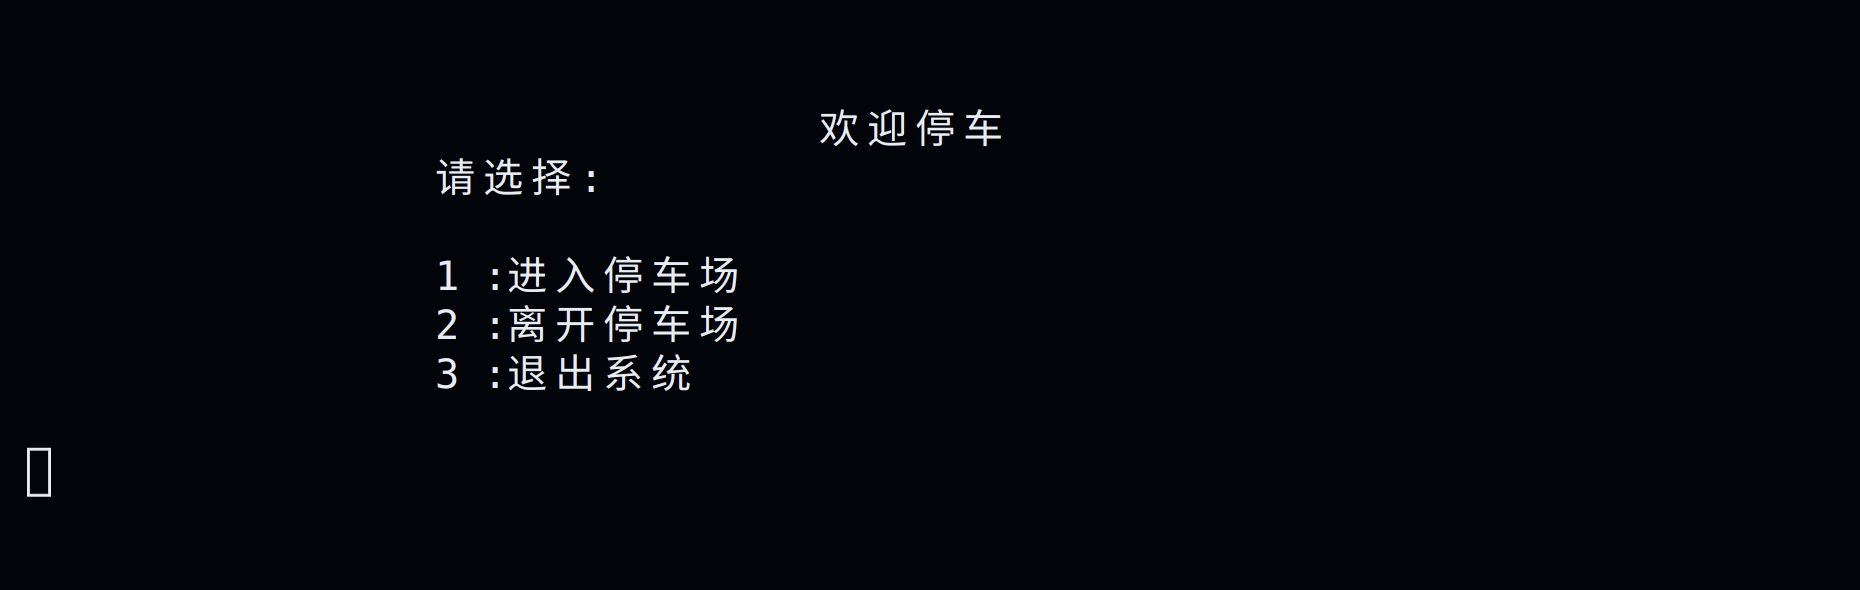
\includegraphics{./fig/parking_2.png}}
         \caption{停车场管理系统演示程序控制台}
         \label{}
        \end{figure}
    }
    \item 输入 1 输入相应信息后,即可完成停车操作
    \item 输入 2 离开即可计算出费用
    \item 输入 3 即可退出系统
\end{enumerate}

\subsection{测试结果}
\begin{enumerate}
    \item 输入 1,车牌号 123456,以及到达时间 2:00
    \item 输入 1,车牌号 654321,以及到达时间 3:00{
        \begin{figure}[H]
        \centering
         \resizebox{0.75\textwidth}{!}{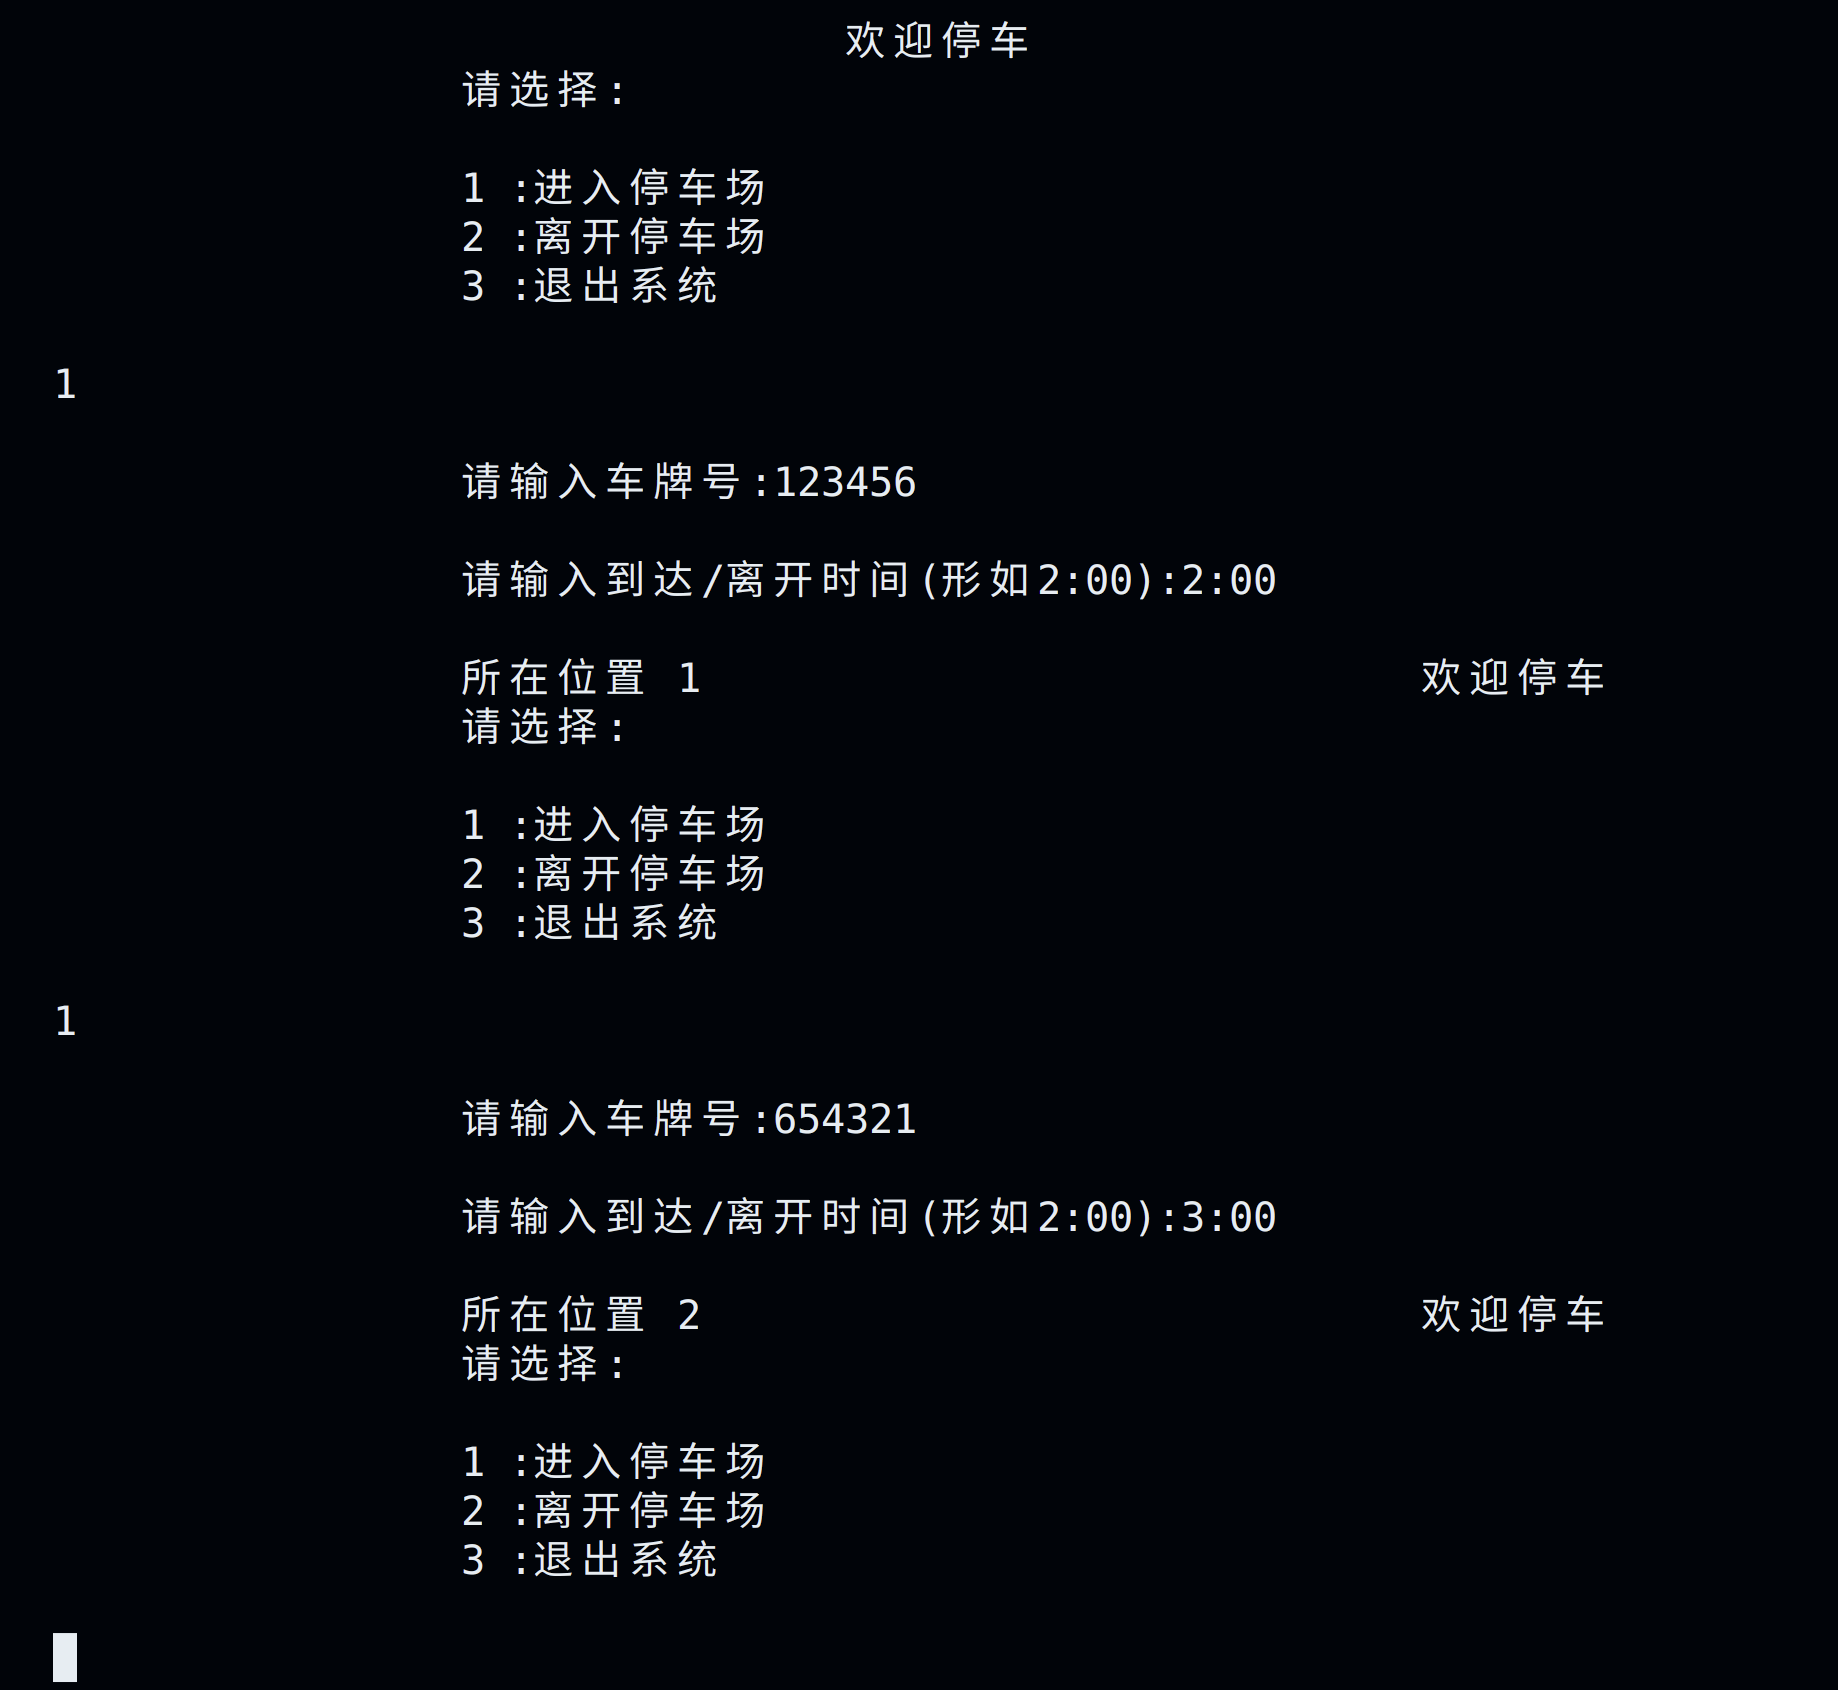
\includegraphics{./fig/parking_r1.png}}
         \caption{输入测试}
         \label{}
        \end{figure}
    }
    \item 输入 2,输入车牌号 123465,输入离开时间 3:00
    \item 输入 2,输入车牌号 654321,输入离开时间 4:00{
        \begin{figure}[H]
        \centering
         \resizebox{0.75\textwidth}{!}{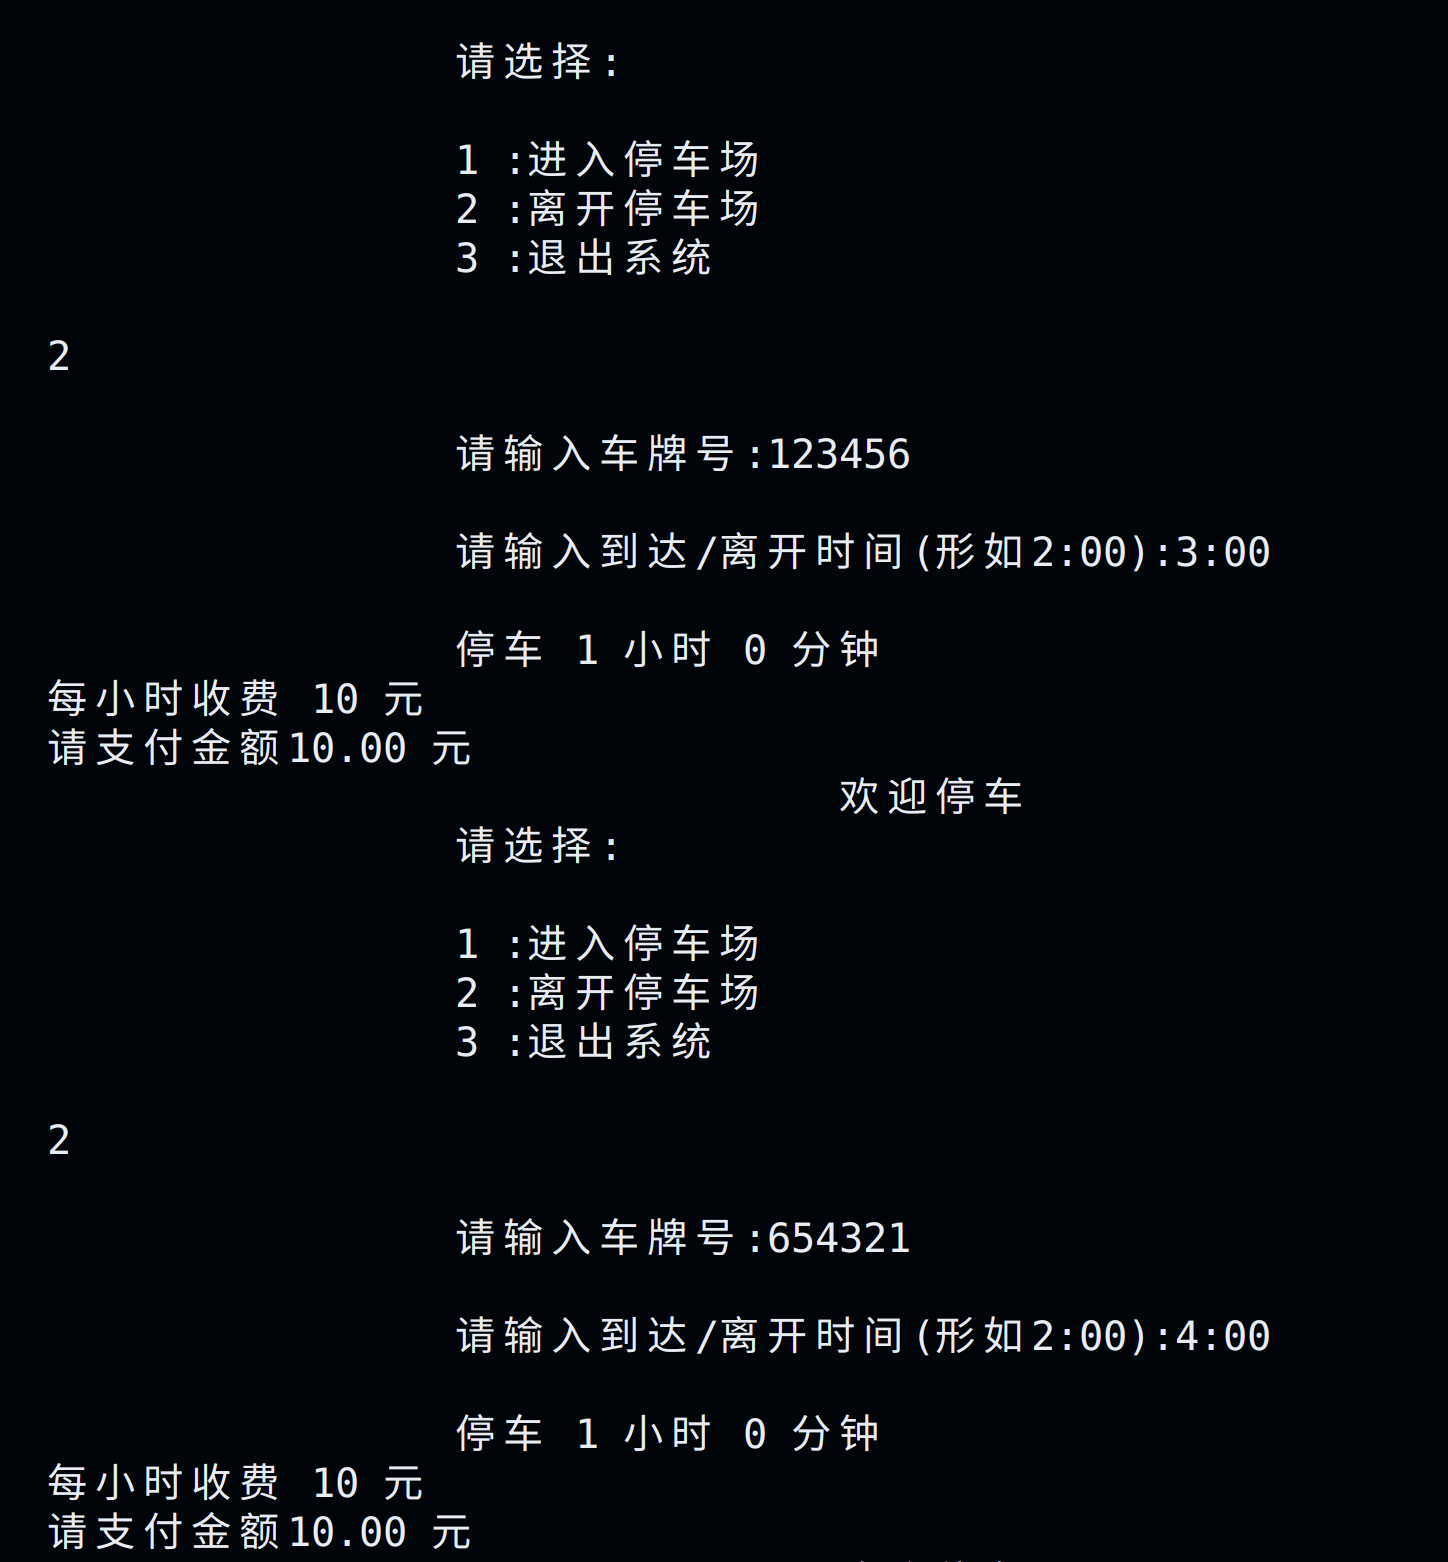
\includegraphics{./fig/parking_r2.png}}
         \caption{输出测试}
         \label{}
        \end{figure}
    }
    \item 测试便道停车功能{
        \begin{figure}[H]
        \centering
         \resizebox{0.75\textwidth}{!}{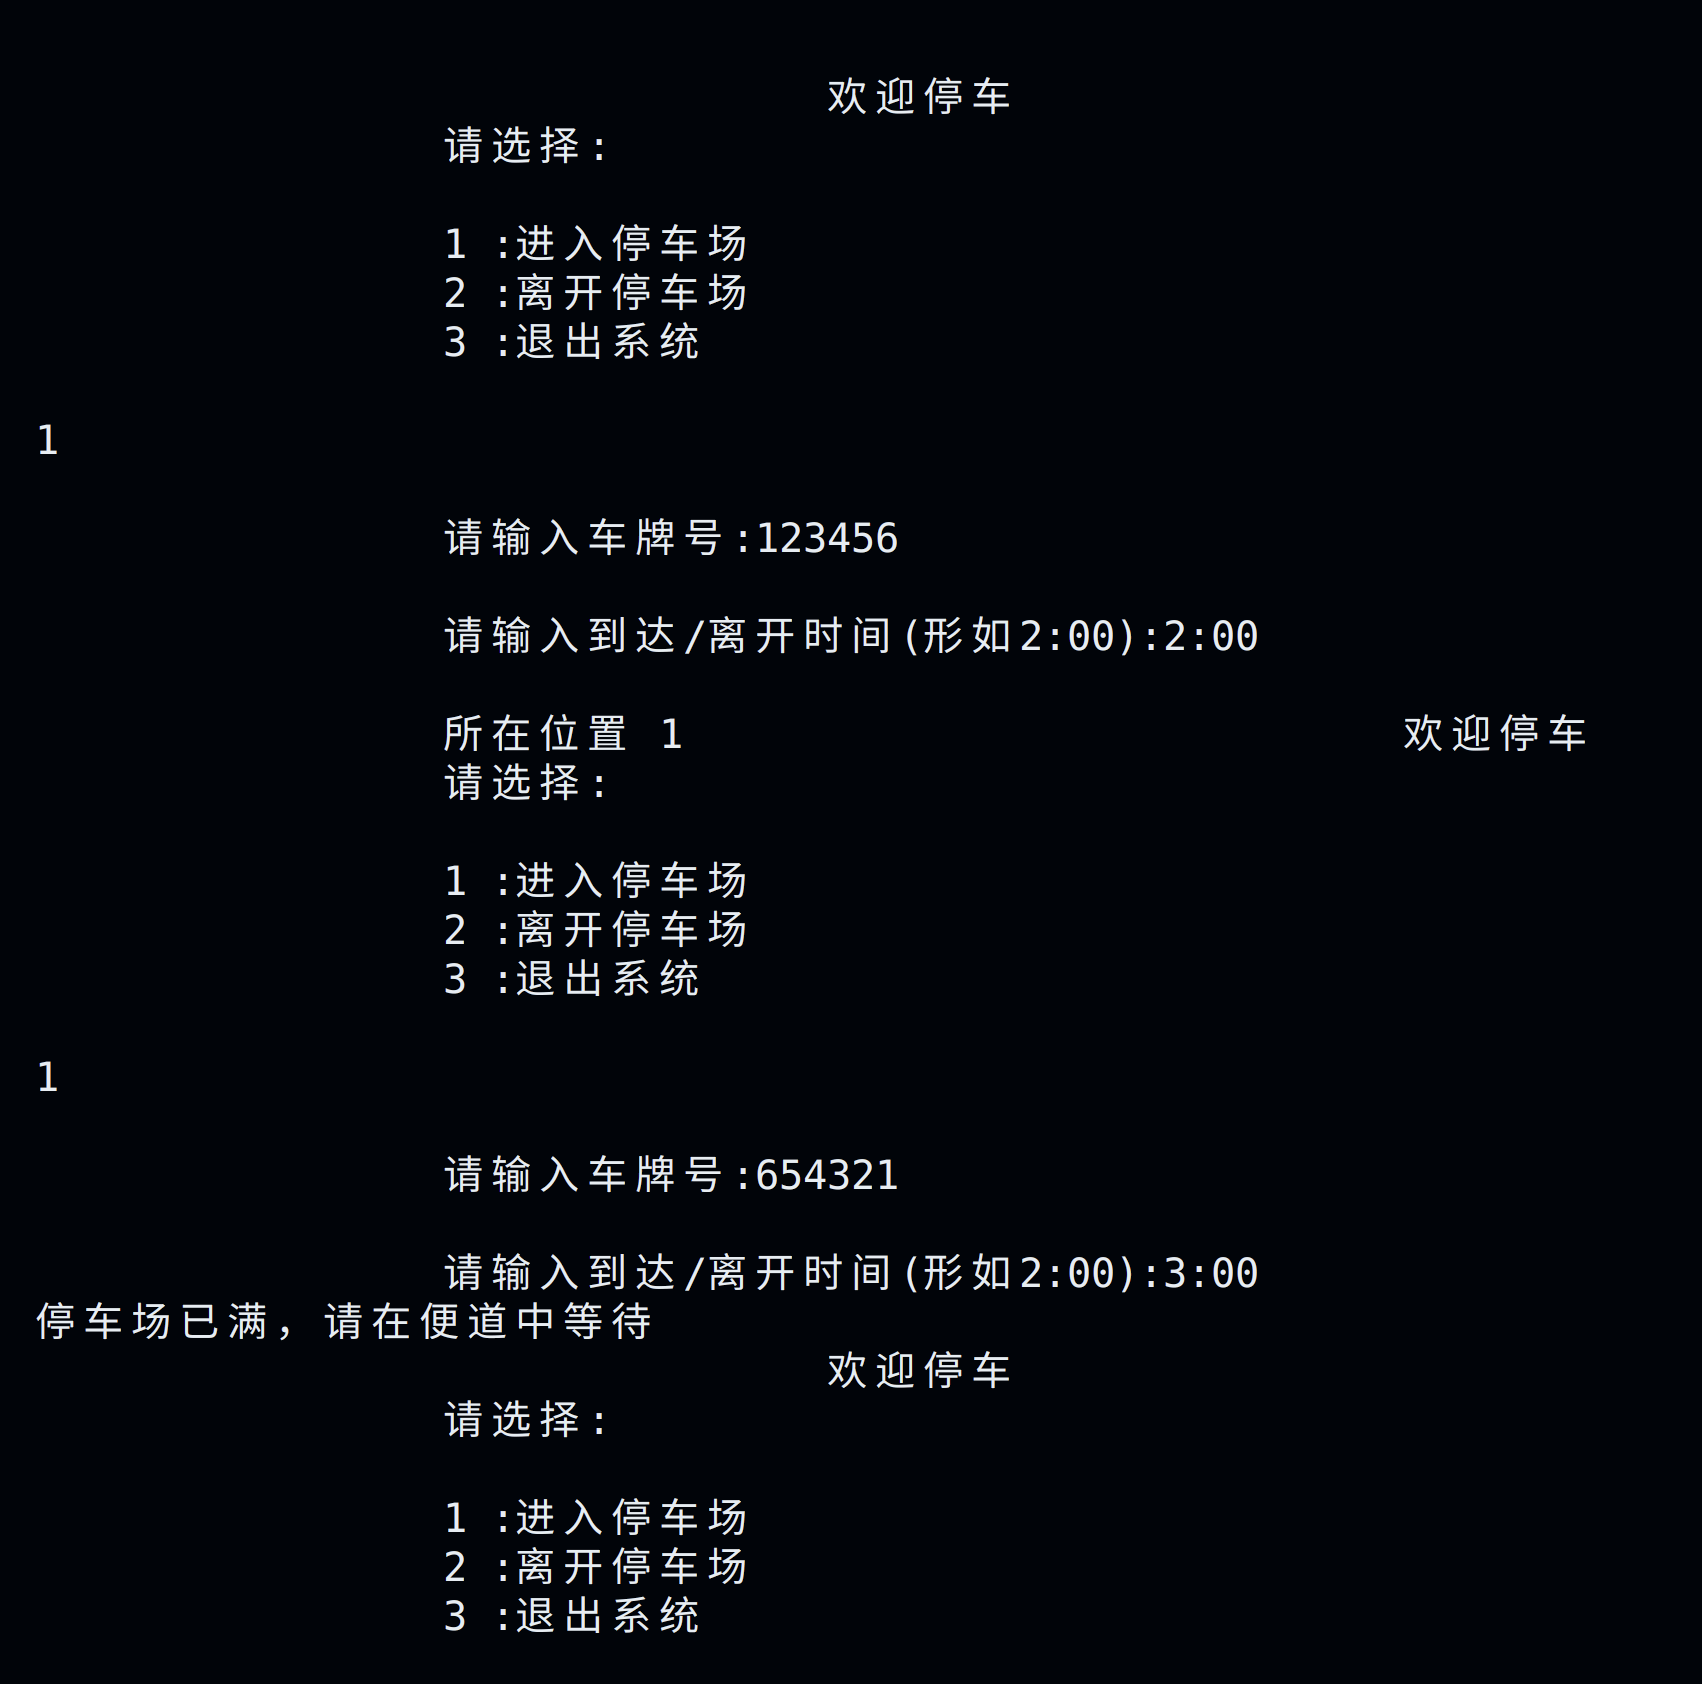
\includegraphics{./fig/parking_r3.png}}
         \caption{测试便道停车功能}
         \label{}
        \end{figure}
    }
\end{enumerate}

\subsection{总结}
本次实验中,我学习了栈和队列的相关知识,掌握了栈和队列的基本操作,以及如何使用栈和队列解决实际问题。在实验过程中,我遇到了一些问题,如何正确的使用栈和队列,如何正确的初始化栈和队列,如何正确的判断栈和队列是否为空,如何正确的判断栈和队列是否为满,如何正确的入栈和出栈,如何正确的入队和出队等等。通过本次实验,我对栈和队列有了更深刻的理解,对栈和队列的操作也更加熟练。

\clearpage
\section{课题三:迷宫问题}

\subsection{任务描述}
迷宫问题是取自心理学的一个古典实验。实验中,把一只老鼠从一个没有顶
的大盒子的门放入,在盒中设置了许多墙,对行进的方向形成了多处阻挡。盒子
仅仅有一个出口,在出口处放置了一块奶酪,吸引老鼠在迷宫中寻找道路以到达
出口。重复对老鼠进行上述实验,看老鼠能在多久找到出口。
请设计一个算法实现迷宫问题求解。

\subsection{功能要求}

找到迷宫中的一条通路,从入口到出口,或者确定没有通路。

\subsection{需求分析}
在对迷宫问题进行建模时,传统的深度优先搜索(DFS)和广度优先搜索(BFS)常常被用作求解策略。然而,这两种方法虽然可以解决问题,但它们并不完全符合现实世界中老鼠寻找奶酪的行为特征。DFS和BFS都属于盲目搜索,需要提前知道整个迷宫的信息,但现实中的老鼠并不可能掌握这样的全局信息。老鼠并不知道迷宫的大小或边界,它所知道的只是在哪个方向上能闻到奶酪的气味,以及前面是否有墙。因此,我考虑使用Q-learning算法最大程度上贴合题意同时解决问题。

Q-learning是一种模型无关的强化学习算法,这意味着该算法并不需要对环境有先验知识,例如它不需要知道地图的边界,这与老鼠的实际行为相匹配。老鼠在寻找奶酪的过程中,并不会事先知道整个迷宫的布局,也就是说,它不知道地图的边界在哪里,或者不知道奶酪在迷宫的哪个位置。

老鼠通过尝试不同的行动和感知环境的反馈,来学习如何在迷宫中找到奶酪。这与Q-learning算法中的探索(Exploration)和利用(Exploitation)的概念非常相似。老鼠会在探索和利用之间做出平衡,尝试新的行动来探索迷宫,同时利用已知的信息来找到奶酪。

至于老鼠能够感知到奶酪的气味,我们可以将其理解为环境给予的奖励(Reward)。在Q-learning算法中,当老鼠在迷宫中移动并最终找到奶酪时,它会得到一定的奖励,这就相当于感知到奶酪的气味。这样,老鼠会学习到一种策略(Policy),指导它如何从起点找到奶酪。

\subsection{概要设计}
程序基本结构设计如下:
\begin{figure}[H]
\centering
 \resizebox{0.75\textwidth}{!}{\includegraphics{./fig/code_structure.jpg}}
 \caption{程序结构}
 \label{}
\end{figure}

各部分叙述如下:
\begin{enumerate}
    \item \textbf{全局变量定义}:在代码的开头定义了一些全局变量,如学习率、折扣因子、迭代次数、epsilon以及每次迭代的最大步数等。这些全局变量在整个程序中被多次使用。
    \item \textbf{迷宫和动作定义}:定义了迷宫的大小、起点和终点,以及可执行的动作。动作被定义为一个二维数组,表示各个方向的移动。
    \item \textbf{函数定义}{
        \begin{enumerate}
            \item[$\bullet$] \textbf{isValidMove}:检查给定的行和列是否是迷宫中的有效位置。
            \item[$\bullet$] \textbf{chooseAction}:基于当前的状态和Q值,选择一个动作。这个动作可以是随机的(探索),也可以是当前Q值最高的(利用)。
            \item[$\bullet$] \textbf{updateQValues}:更新Q值表。新的Q值是基于旧的Q值、当前的奖励和最大可能的未来奖励计算的。
            \item[$\bullet$] \textbf{qLearning}:实现Q-learning算法的主体部分。首先,初始化Q值表,然后进行多次迭代。在每次迭代中,从起点开始,选择并执行动作,然后更新Q值,直到到达终点或达到最大步数。迭代结束后,选择Q值最高的动作,找到从起点到终点的路径。
        \end{enumerate}
    }
    \item \textbf{主函数}:主函数首先从文件读入迷宫的数据,然后调用\textbf{qLearning}函数进行学习和找路径。最后,返回0表示程序正常结束。 
\end{enumerate}

\subsection{详细设计}
Q-learning 代码
\begin{minted}[linenos]{c++}
    #include <bits/stdc++.h> // 引入常用库

    // 定义强化学习的一些参数
    const double learningRate = 0.9;     // 学习率
    const double discountFactor = 0.9;   // 折扣因子
    const int numEpisodes = 5000;        // 总的训练轮数
    double epsilon = 0.9;                // ε-贪婪策略中的参数
    const double epsilonDecay = 0.99;    // ε的衰减系数
    const int maxStepsPerEpisode = 3000; // 每轮训练的最大步数
    
    // 定义迷宫的相关参数
    int numRows = 6;                    // 迷宫的行数
    int numCols = 5;                    // 迷宫的列数
    std::vector<std::vector<int>> maze; // 二维向量表示的迷宫,0表示通道,1表示墙
    
    // 定义起点和终点
    int startRow = 0;         // 起点的行坐标
    int startCol = 0;         // 起点的列坐标
    int endRow = numRows - 1; // 终点的行坐标
    int endCol = numCols - 1; // 终点的列坐标
    
    // 定义8种可能的行动:上、下、左、右、左上、右上、左下、右下
    int actions[8][2] = {{-1, 0},  {1, 0},  {0, -1}, {0, 1},
                         {-1, -1}, {-1, 1}, {1, -1}, {1, 1}};
    int action_cnt = 8; // 行动的种类数
    
    // 判断是否是合法的移动
    bool isValidMove(int row, int col) {
      if (row >= 0 && row < numRows && col >= 0 && col < numCols &&
          maze[row][col] == 0) {
        return true;
      }
      return false;
    }
    
    // 根据当前状态和Q值表选择行动
    int chooseAction(int row, int col,
                     std::vector<std::vector<std::vector<double>>> &qValues,
                     int previousAction) {
      // epsilon-greedy策略选择动作
    
      double random =
          static_cast<double>(rand()) / RAND_MAX; // 生成一个[0, 1)之间的随机数
      if (random < epsilon) {                  // 以ε的概率随机选择动作
        std::vector<int> validActions;         // 存储所有有效的动作
        for (int i = 0; i < action_cnt; i++) { // 遍历所有可能的动作
          int newRow = row + actions[i][0];    // 计算执行动作后的新位置
          int newCol = col + actions[i][1];
          if (isValidMove(newRow, newCol)) { // 如果该动作是有效的
            validActions.push_back(i); // 将该动作加入到有效动作列表中
          }
        }
    
        if (validActions.empty()) { // 如果没有有效的动作
          return -1;                // 返回-1表示无有效动作
        }
    
        return validActions[rand() %
                            validActions.size()]; // 在所有有效动作中随机选择一个
      }
    
      // 以1-ε的概率选择最优的动作
      int bestAction = -1;                   // 存储最优动作
      double maxValue = -1e9;                // 存储最大的Q值
      for (int i = 0; i < action_cnt; i++) { // 遍历所有可能的动作
        int newRow = row + actions[i][0];    // 计算执行动作后的新位置
        int newCol = col + actions[i][1];
        // 如果该动作是有效的并且Q值大于当前最大的Q值,那么更新最优动作和最大Q值
        if (isValidMove(newRow, newCol) && qValues[row][col][i] > maxValue &&
            (previousAction == -1 || // 对于第一步,任何动作都可以是最优动作
             (actions[i][0] !=
                  -actions[previousAction][0] || // 不选取与上一步相反的动作
              actions[i][1] != -actions[previousAction][1]))) {
          maxValue = qValues[row][col][i];
          bestAction = i;
        }
      }
      return bestAction; // 返回最优动作
    }
    
    // 根据公式更新Q值表
    void updateQValues(int currentRow, int currentCol, int newRow, int newCol,
                       int action,
                       std::vector<std::vector<std::vector<double>>> &qValues) {
      double maxQValue = -1e9;               // 存储最大的Q值
      for (int i = 0; i < action_cnt; i++) { // 遍历所有可能的动作
        // 如果Q值大于当前最大的Q值,那么更新最大Q值
        if (qValues[newRow][newCol][i] > maxQValue) {
          maxQValue = qValues[newRow][newCol][i];
        }
      }
    
      // 定义奖励值,如果到达目标位置则奖励为100,否则按离终点的距离给予惩罚
      double distance=sqrt(pow(newRow - endRow, 2) + pow(newCol - endCol, 2));
      double reward = (distance == 0) ? 100 : -distance;
      // 根据Q学习算法的公式更新Q值
      qValues[currentRow][currentCol][action] +=
          learningRate * (reward + discountFactor * maxQValue -
                          qValues[currentRow][currentCol][action]);
    }
    
    // Q学习的主要函数
    void qLearning() {
      srand(time(0)); // 设置随机种子
      // 初始化Q值表,所有的Q值都设置为0
      std::vector<std::vector<std::vector<double>>> qValues(
          numRows, std::vector<std::vector<double>>(
                       numCols, std::vector<double>(action_cnt, 0)));
    
      // 进行numEpisodes轮训练
      for (int episode = 0; episode < numEpisodes; episode++) {
        int currentRow = startRow; // 当前位置的行坐标
        int currentCol = startCol; // 当前位置的列坐标
    
        int step = 0;            // 计步器
        int previousAction = -1; // 上一步的动作
        // 当未达到目标且未超过每轮最大步数时,继续训练
        while ((currentRow != endRow || currentCol != endCol) &&
               step < maxStepsPerEpisode) {
          // 选择一个动作
          int action = chooseAction(currentRow, currentCol, qValues, -1);
    
          if (action == -1) { // 如果没有有效的动作
            break;            // 结束本轮训练
          }
    
          // 执行选定的动作,更新当前位置
          int newRow = currentRow + actions[action][0];
          int newCol = currentCol + actions[action][1];
    
          if (isValidMove(newRow, newCol)) { // 如果移动后的位置有效
            // 更新Q值表
            updateQValues(currentRow, currentCol, newRow, newCol, action, qValues);
            currentRow = newRow; // 更新当前位置
            currentCol = newCol;
            previousAction = action; // 更新上一步的动作
          }
          step++; // 计步器增加
        }
        // ε按衰减系数衰减
        epsilon *= epsilonDecay;
      }
    
      double originalEpsilon = epsilon; // 存储原始的ε值
      epsilon = 0; // ε设为0,即在路径规划时只采用贪婪策略
    
      // 显示找到的路径
      std::vector<std::pair<int, int>> path; // 存储路径
      int currentRow = startRow;             // 当前位置的行坐标
      int currentCol = startCol;             // 当前位置的列坐标
      path.push_back(std::make_pair(currentRow, currentCol)); // 将起点加入到路径中
      int previousAction1 = -1;                               // 上一步的动作
    
      while (currentRow != endRow ||
             currentCol != endCol) { // 当未到达终点时,继续行走
        // 选择最优动作
        int bestAction =
            chooseAction(currentRow, currentCol, qValues, previousAction1);
    
        if (bestAction == -1) { // 如果没有有效的动作
          std::cout << "There is no valid path!" << std::endl; // 输出提示信息
          return;                                              // 结束函数执行
        }
    
        // 执行选定的动作,更新当前位置
        int newRow = currentRow + actions[bestAction][0];
        int newCol = currentCol + actions[bestAction][1];
    
        if (isValidMove(newRow, newCol)) { // 如果移动后的位置有效
          currentRow = newRow;             // 更新当前位置
          currentCol = newCol;
          path.push_back(
              std::make_pair(currentRow, currentCol)); // 将新位置加入到路径中
          previousAction1 = bestAction;                // 更新上一步的动作
        }
      }
    
      // 输出找到的路径
      for (const auto &p : path) {
        std::cout << "(" << p.first << ", " << p.second << ") ";
      }
      std::cout << std::endl;
    
      // 恢复原始的ε值
      epsilon = originalEpsilon;
    }
    
    // 主函数
    int main() {
      // 从文件读取迷宫数据
      freopen("/media/zby/SSD数据盘/Program-Practice/Maze/build/maze.txt", "r",
              stdin);
      std::cin >> numRows >> numCols; // 输入迷宫的行数和列数
      maze.resize(numRows, std::vector<int>(numCols)); // 调整迷宫大小
      for (int i = 0; i < numRows; i++) {              // 输入迷宫数据
        for (int j = 0; j < numCols; j++) {
          std::cin >> maze[i][j];
        }
      }
    
      qLearning(); // 执行Q学习算法
    
      return 0; // 程序结束
    }
    
    
\end{minted}

附上一开始写的DFS版本

\begin{minted}[linenos]{c++}
    #include <iostream>
    #include <vector>
    #include <stack>
    
    // 定义迷宫的相关参数
    int numRows = 6;                    // 迷宫的行数
    int numCols = 5;                    // 迷宫的列数
    std::vector<std::vector<int>> maze; // 二维向量表示的迷宫,0表示通道,1表示墙
    
    // 定义8种可能的行动:上、下、左、右、左上、右上、左下、右下
    int actions[8][2] = {{-1, 0},  {1, 0},  {0, -1}, {0, 1},
                         {-1, -1}, {-1, 1}, {1, -1}, {1, 1}};
    int action_cnt = 8; // 行动的种类数
    
    // 判断是否是合法的移动
    bool isValidMove(int row, int col) {
      if (row >= 0 && row < numRows && col >= 0 && col < numCols &&
          maze[row][col] == 0) {
        return true;
      }
      return false;
    }
    
    // 使用深度优先搜索解决迷宫问题
    bool dfs(int currentRow, int currentCol, std::vector<std::vector<bool>>& visited,
             std::vector<std::pair<int, int>>& path) {
      // 到达终点,返回true
      if (currentRow == numRows - 1 && currentCol == numCols - 1) {
        return true;
      }
    
      visited[currentRow][currentCol] = true; // 将当前位置标记为已访问
    
      // 遍历所有可能的动作
      for (int i = 0; i < action_cnt; i++) {
        int newRow = currentRow + actions[i][0]; // 计算执行动作后的新位置
        int newCol = currentCol + actions[i][1];
    
        // 如果新位置是合法的且未被访问过
        if (isValidMove(newRow, newCol) && !visited[newRow][newCol]) {
          // 将新位置加入到路径中
          path.push_back(std::make_pair(newRow, newCol));
    
          // 递归调用DFS搜索
          if (dfs(newRow, newCol, visited, path)) {
            return true; // 如果找到一条路径,返回true
          }
    
          // 未找到路径,回溯
          path.pop_back();
        }
      }
    
      return false; // 未找到路径,返回false
    }
    
    // 解决迷宫问题的主函数
    void solveMaze() {
      // 创建一个二维布尔数组来记录访问状态
      std::vector<std::vector<bool>> visited(numRows, std::vector<bool>(numCols, false));
    
      std::vector<std::pair<int, int>> path; // 存储路径
      path.push_back(std::make_pair(0, 0));  // 将起点加入到路径中
    
      if (dfs(0, 0, visited, path)) {
        // 输出找到的路径
        for (const auto& p : path) {
          std::cout << "(" << p.first << ", " << p.second << ") ";
        }
        std::cout << std::endl;
      } else {
        std::cout << "There is no valid path!" << std::endl;
      }
    }
    
    int main() {
      // 从文件读取迷宫数据
      freopen("/media/zby/SSD数据盘/Program-Practice/Maze/build/maze.txt", "r", stdin);
      std::cin >> numRows >> numCols; // 输入迷宫的行数和列数
      maze.resize(numRows, std::vector<int>(numCols)); // 调整迷宫大小
      for (int i = 0; i < numRows; i++) {              // 输入迷宫数据
        for (int j = 0; j < numCols; j++) {
          std::cin >> maze[i][j];
        }
      }
    
      solveMaze(); // 解决迷宫问题
    
      return 0; // 程序结束
    }
    
\end{minted}
\subsection{调试分析}
\begin{enumerate}
    \item 一开始写了dfs版本,但是因为太简单了所以改用qlearning了
    \item 开始的时候因为以为题意是四方向移动,发现当无解的时候程序会死循环,因此加入了最大步数的限制,因此后来改成了八方向移动,这样就不会出现死循环的情况了。
    \item 一开始考虑奖励函数设为到终点为100其余为-1,后考虑老鼠离终点越近奖励越大,因此改成了距离终点的距离,这样老鼠就会尽可能的走向终点。
    \item 一开始地图直接在程序中定义,但是调整迷宫不方便,因此改成了从文件中读取迷宫数据。
\end{enumerate}

\subsection{用户手册}
演示程序的运行环境为Ubuntu 20.04,编译器为g++ 9.4.0,编译选项为-O,Q-learning的执行指令为
\begin{minted}{c}
    cd "/media/zby/SSD数据盘/Program-Practice/Maze/" 
    && g++ main.cpp -o main 
    && "/media/zby/SSD数据盘/Program-Practice/Maze/"main"
\end{minted}

DFS的执行指令为
\begin{minted}{c}
    cd "/media/zby/SSD数据盘/Program-Practice/Maze/" 
    && g++ dfs.cpp -o dfs 
    && "/media/zby/SSD数据盘/Program-Practice/Maze/"dfs"
\end{minted}
\emph{$\star$迷宫文件的格式为:第一行为迷宫的行数和列数,接下来的行数为迷宫的数据,0表示通道,1表示墙,如下所示。}
\begin{figure}[H]
\centering
 \resizebox{0.25\textwidth}{!}{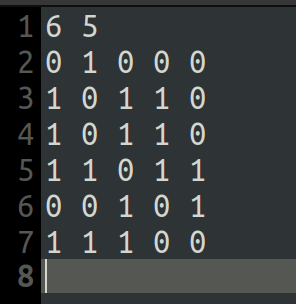
\includegraphics{./fig/maze.png}}
 \caption{迷宫样例数据}
 \label{}
\end{figure}

\subsection{测试结果}
\begin{figure}[H]
\centering
 \resizebox{1\textwidth}{!}{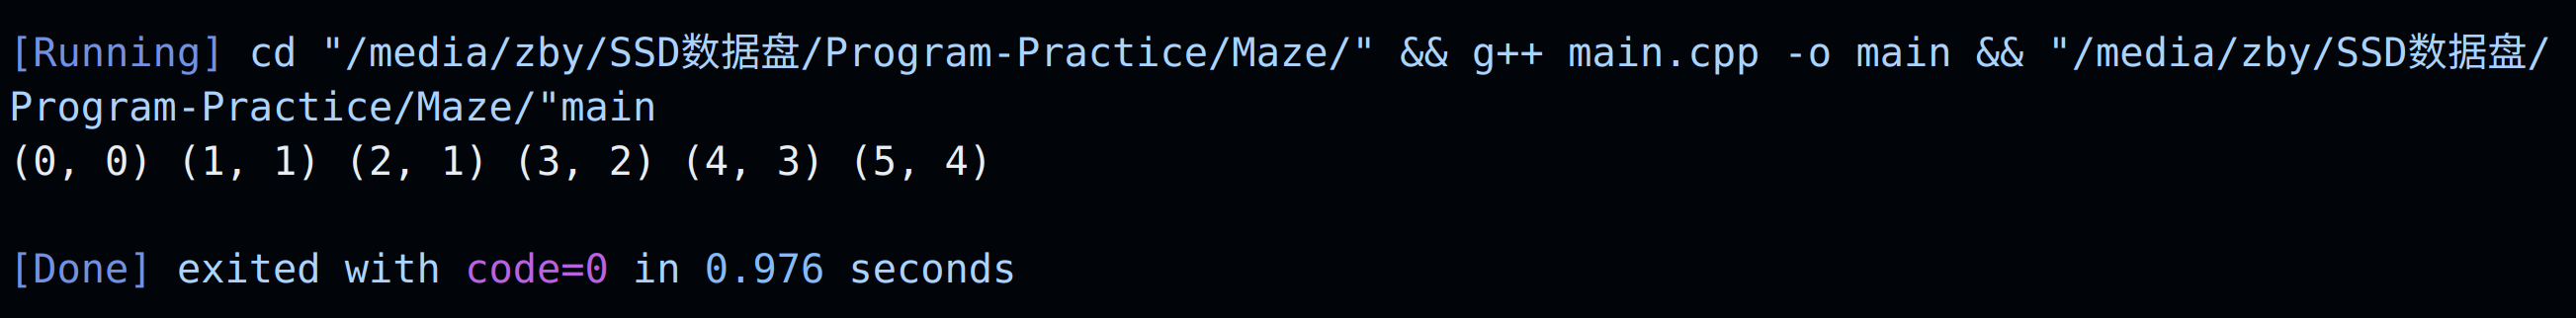
\includegraphics{./fig/maze_r1.png}}
 \caption{迷宫有解情况(Q-learning)}
 \label{}
\end{figure}

\begin{figure}[H]
\centering
 \resizebox{1\textwidth}{!}{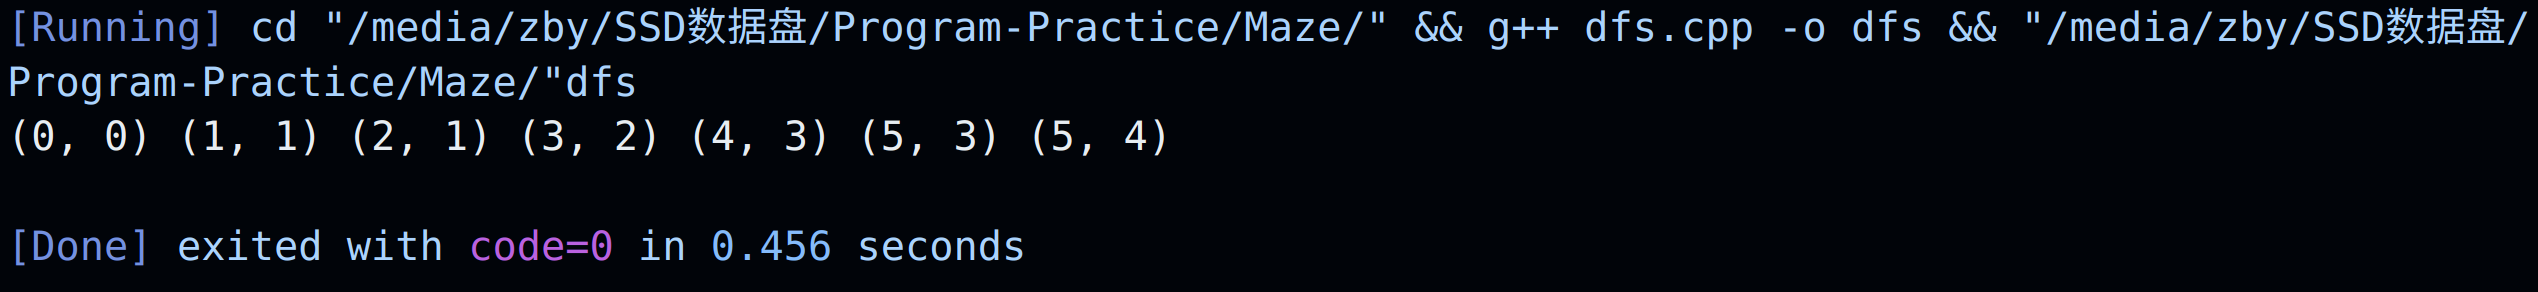
\includegraphics{./fig/maze_dfs.png}}
 \caption{迷宫有解情况(DFS)}
 \label{}
\end{figure}
\begin{figure}[H]
\centering
 \resizebox{1\textwidth}{!}{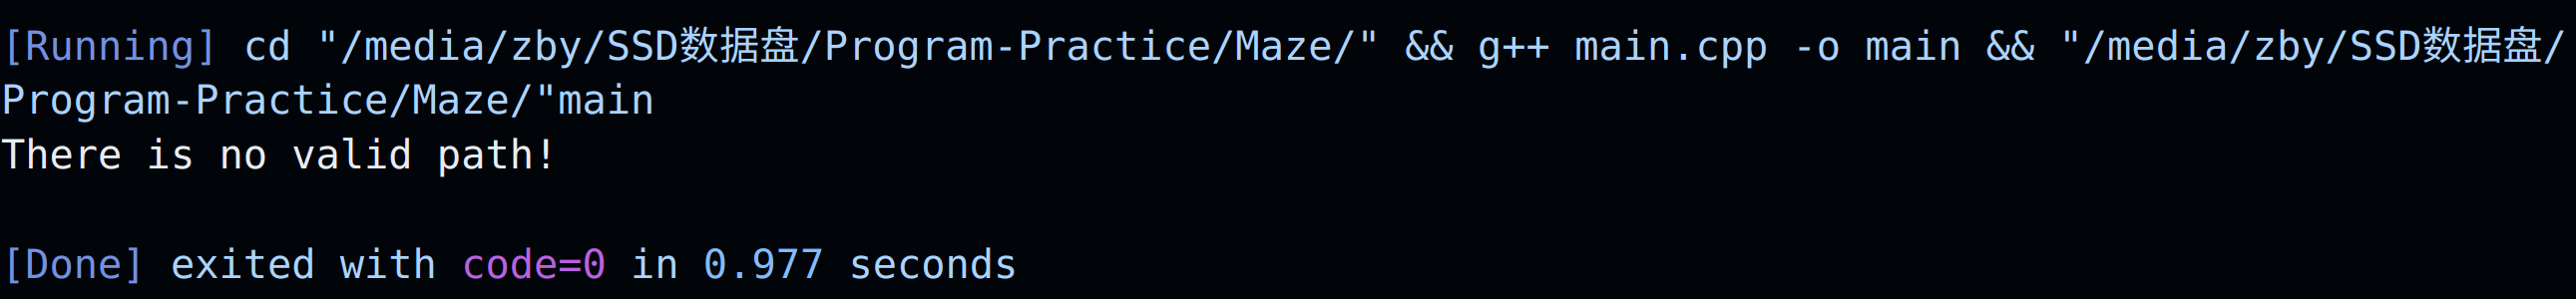
\includegraphics{./fig/maze_err.png}}
 \caption{迷宫无解情况}
 \label{}
\end{figure}

\subsection{总结与分析}
Q学习算法和深度优先搜索算法在解决迷宫问题上有着不同的特点。Q学习算法是一种基于强化学习的方法,通过训练和学习来得到最优策略。它能够找到最优路径,但需要预先训练并更新Q值表。深度优先搜索算法是一种盲目搜索方法,通过穷举所有可能的路径来找到一条路径。它能够找到路径,但不保证是最优路径,且没有训练过程。

选择哪种算法取决于具体的需求和问题情况。如果希望找到最优路径,并且有足够的训练数据和时间进行学习,那么Q学习算法是一个好的选择。
如果只需要找到任意可行的路径,并且不需要训练过程,那么深度优先搜索算法是一个简单且有效的方法。
在实际应用中,根据问题的特点和要求,可以选择适合的算法来解决迷宫问题,或者结合两种算法的优点进行改进和优化。

\clearpage

\end{document}